\section{Introduction} \label{SciRob:sec:intro}

Control and motion planning methods that rely on models to predict the outcomes of potential actions are ubiquitous in robotics. But whether these models are analytical, simulated, learned, or implicit within a policy, they are only as valid as the assumptions used to create them. When encountering a real-world unstructured environment, these assumptions may be violated, rendering a model unreliable \cite{Wang2019}. What is worse, estimating how erroneous our models are is difficult, as methods that predict uncertainty distributions based on training data \cite{Chua2018,Lakshminarayanan2017} don’t account for novel scenarios, e.g. when new types of constraints are introduced. This is especially problematic if these constraints are not easily represented \cite{Kamthe2018} in the model’s state space. Consequently, the inability to generate meaningful predictive uncertainty distributions for novel scenarios precludes the use of belief-space planning techniques \cite{WangBounded2018,FIRM,LQGMP}.

Roboticists rarely address the unreliable model problem directly; instead, we often resort to high-frequency re-planning, hoping to compensate for model errors online \cite{Finn2017,Koller2019}. But this kind of approach assumes that the erroneous model is somehow likely to produce useful short-horizon actions. While it may not be possible to create universally-valid models of complex high-degree-of-freedom systems such as deformable objects, this does not preclude using imperfect models to perform useful tasks. For example, we do not need to know all the friction and stiffness properties of a rope to drag it along the ground. The key questions, which have, until now, received very little attention, are \textit{1) When should we trust a model?} and \textit{2) What do we do if the robot is in a state where the model is unreliable?} Addressing these questions is paramount if we wish to deploy robots in unstructured environments such as homes and industrial sites, where conditions change frequently, and it may not be possible to gather large datasets and re-learn accurate dynamics after every change. 

This paper tackles the above two questions in the context of learning dynamics models for the manipulation of rope-like objects among constraints such as obstacles. A key challenge in this domain is that the behavior of the rope when in contact is extremely difficult to predict, as it is heavily influenced by the rope’s often non-uniform friction and stiffness properties. These properties are not only difficult to model, they are also difficult to estimate from observation. Thus, the hypothesis at the core of our work is that it is much better to learn to predict where a useful (but limited) model is reliable than to attempt to learn a model which is reliable everywhere. Specifically, in the context of rope manipulation, we propose a two-phase learning process, where we learn a useful model of rope dynamics assuming constraints such as obstacles are not present. Then, given limited data of the rope’s interaction with obstacles, we can learn a classifier that predicts when the learned model is reliable. We then use this classifier in motion planning for novel tasks to bias the planner away from regions of state space where the model cannot be trusted. We emphasize that we do not attempt to learn the dynamics of the rope in contact from this limited dataset. In fact, we find that attempting to learn these dynamics yields poor results.

While the above methods allow us to perform useful tasks with rope despite being unable to predict dynamics on constraints boundaries, we are still faced with the question of what to do when the rope strays into a part of state space where the learned model is unreliable. This may occur because of error in execution, an external disturbance, or simply by starting the task in a state from which prediction is unreliable. Our approach for overcoming this problem is to first use our classifier to detect when this has occurred, and then to recover—i.e. execute a series of actions that bring us back to a region where the learned model is reliable. While random actions can eventually lead us to this region, we find that it is more efficient to use a recovery policy (also learned from the limited dataset) to determine which actions are likely to improve model reliability. After reaching the region where our predictions are reliable, we can launch our planner to move to the goal. An overview of our learning and execution frameworks is shown in Figure \ref{Scirob:fig:figure1}.

\begin{figure}
    \centering
    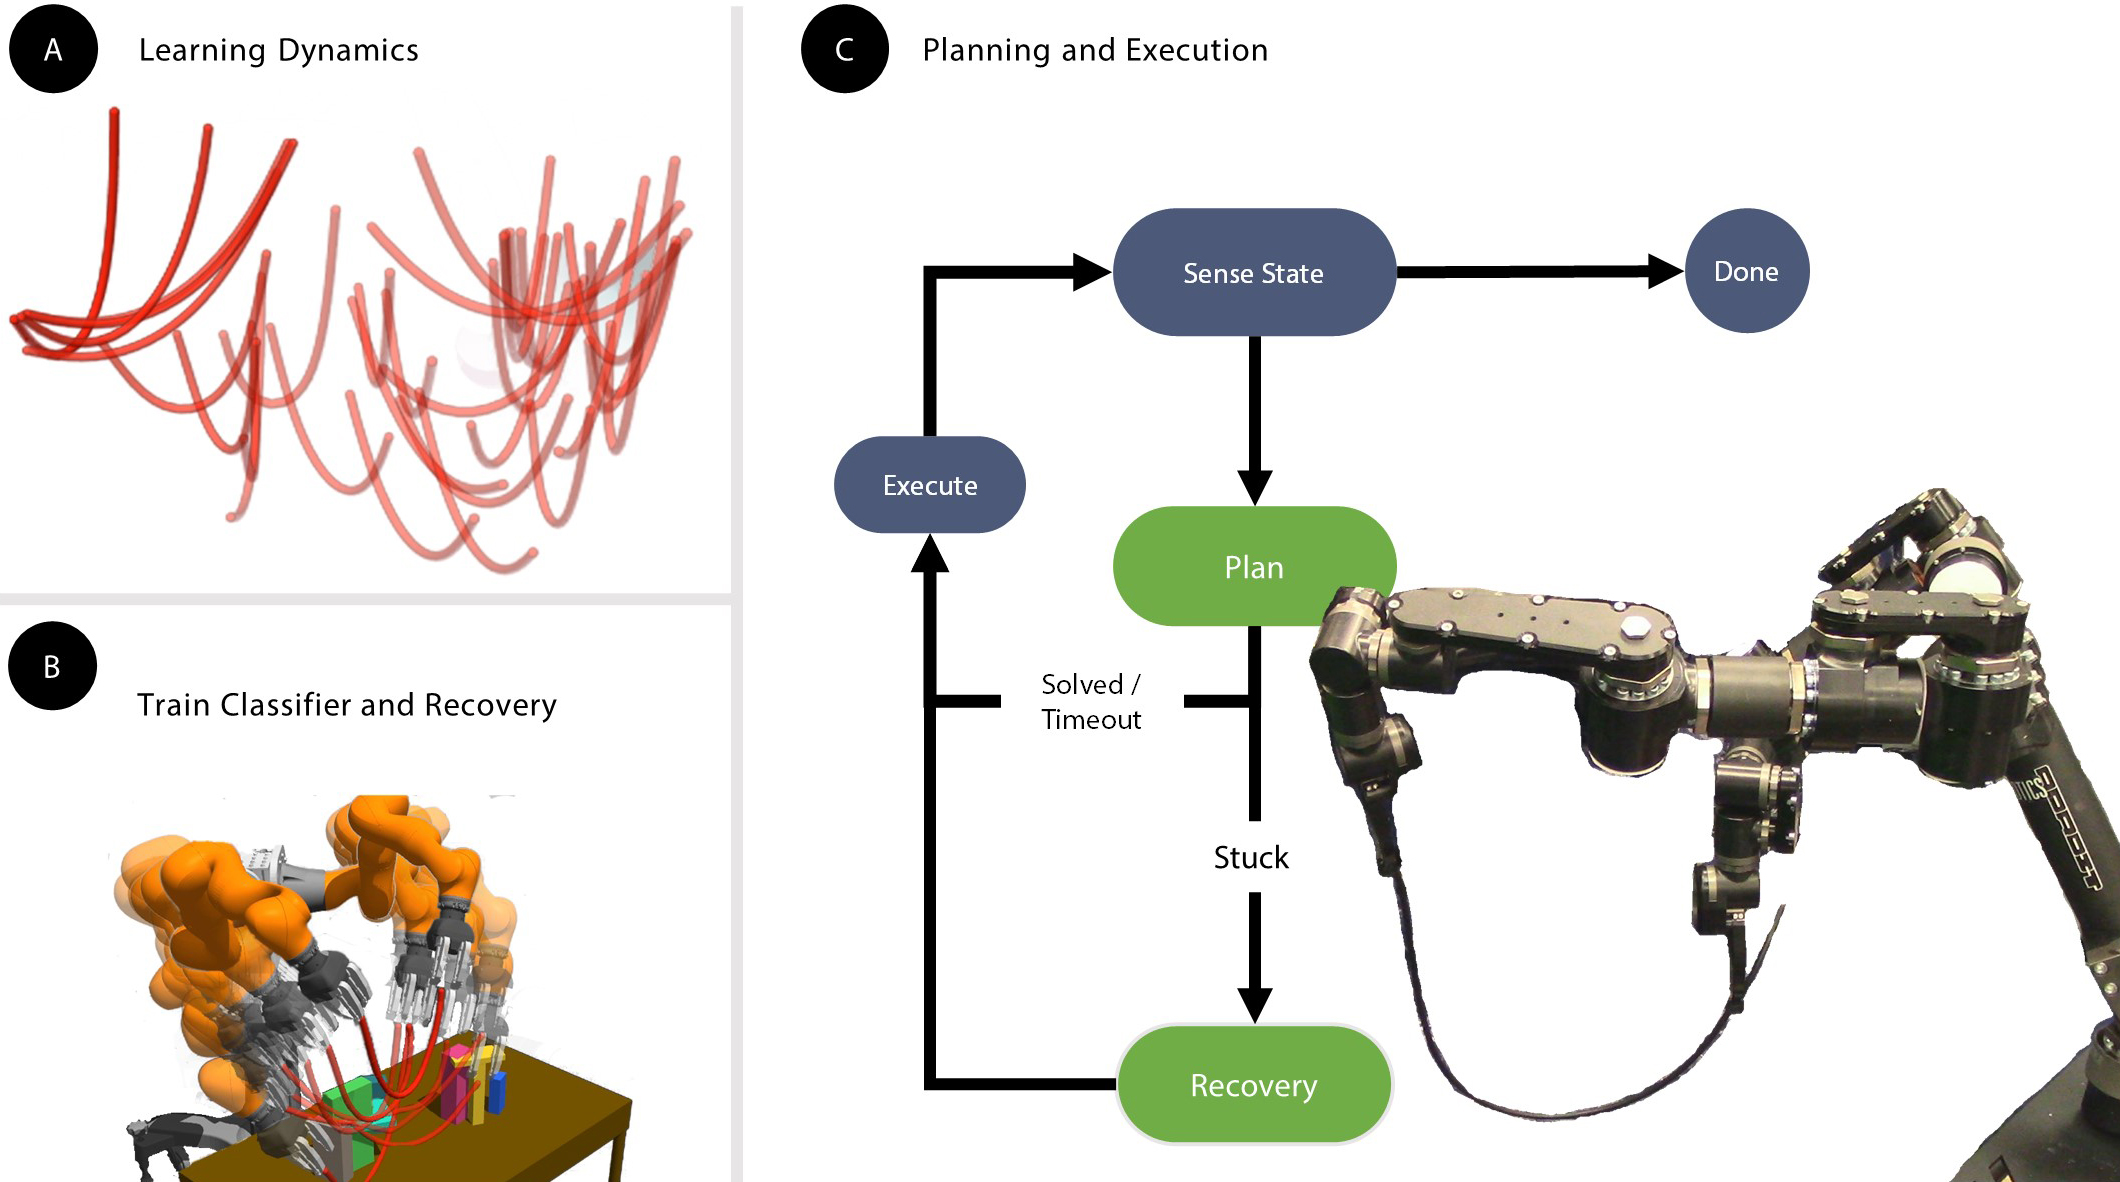
\includegraphics[width=0.8\linewidth]{Chap2/images/figure1}
    \caption{Overview of the proposed method. Two data collection phases (A,B) are used to collect training data for learning dynamics, a classifier for where these dynamics are accurate, and a recovery model what for actions to take when no accurate dynamics predictions can be made. These learned components are used in an iterative process of planning, replanning, and recovery (C). We apply this method to a number of deformable objects tasks, including a dual arm robot manipulating an automotive hose.}
    \label{Scirob:fig:figure1}
\end{figure}